\documentclass[11pt,a4paper]{article}

\usepackage[margin=0.85in]{geometry}
\usepackage{amsmath,amssymb,bm}
\usepackage{booktabs}
\usepackage{array}
\usepackage{hyperref}
\usepackage{graphicx}
\usepackage{pdflscape}

\title{PI-DU-RACE: Sixteen-Stage Spectrum-Adaptive\\
Deep-Unfolded Rydberg Channel Estimator}
\author{}
\date{}

\begin{document}
\maketitle

\section{Purpose and current configuration}

The estimator reconstructs the complex user-channel matrix from
magnitude-only observations. The current frozen comparison uses
\[
N=8,\qquad K=3,\qquad \mathrm{RSR}=25~\mathrm{dB},
\]
with separate models for \(P=10\) and \(P=30\) pilots. The training
SNR grid is
\[
\{-5,0,5,10,15,20,25,30\}~\mathrm{dB}.
\]

The measurement model is
\begin{equation}
\bm{Y}
=
\left|\bm{G}\bm{S}+\bm{B}+\bm{W}\right|,
\end{equation}
where
\[
\bm{G}\in\mathbb{C}^{N\times K},\quad
\bm{S}\in\mathbb{C}^{K\times P},\quad
\bm{B},\bm{W}\in\mathbb{C}^{N\times P},\quad \bm{Y}\in\mathbb{R}_{+}^{N\times P}.
\]
The absolute value is applied elementwise. The receiver observes
\(\bm{Y}\), while the pilots \(\bm{S}\), reference \(\bm{B}\), and noise
variance \(\sigma^2\) are known to the estimator.

The model is physics-informed deep unfolding: each learned stage follows
an EM-GS measurement update, a Hankel-structure refinement, and a learned
gate. It is not a pure black-box network and contains no Transformer
block.



\section{Initialization}

For each observation, a biased-GS iterative estimator creates the initial
channel estimate
\[
\bm{G}^{(0)}\in\mathbb{C}^{N\times K}.
\]
The initialization uses the same magnitude observations and known
measurement inputs. In the current configuration, GS is run for at most
\(5000\) updates with relative-change tolerance \(10^{-10}\).

Thus, the unfolded network begins from a nonlinear GS estimate, not from
a linearized channel estimate.

\section{One unfolded stage}

There are \(T=16\) stages. At stage \(t\), the previous estimate is
\[
\bm{G}^{(t-1)}\in\mathbb{C}^{N\times K}.
\]
The stage creates an EM-GS candidate, a Hankel-refined candidate, and
then combines three candidate estimates using one learned three-branch
softmax gate.

\subsection{1. EM-GS measurement update}

The predicted complex field is
\begin{equation}
\bm{F}^{(t)}
=
\bm{G}^{(t-1)}\bm{S}+\bm{B}
\in\mathbb{C}^{N\times P}.
\end{equation}
For magnitude measurements with complex Gaussian noise, the implementation
forms the concentration parameter
\begin{equation}
\kappa^{(t)}_{np}
=
\frac{2Y_{np}\left|F^{(t)}_{np}\right|}{\sigma^2}.
\end{equation}
The modified-Bessel ratio is
\begin{equation}
R^{(t)}_{np}
=
\frac{I_1\!\left(\kappa^{(t)}_{np}\right)}
     {I_0\!\left(\kappa^{(t)}_{np}\right)}.
\end{equation}
The reconstructed complex observation is
\begin{equation}
U^{(t)}_{np}
=
Y_{np}
\exp\!\left(j\arg F^{(t)}_{np}\right)
R^{(t)}_{np}.
\end{equation}
The EM-GS channel candidate is then
\begin{equation}
\bm{G}_{\mathrm{EM}}^{(t)}
=
\left(\bm{U}^{(t)}-\bm{B}\right)
\bm{S}^{\dagger},
\qquad
\bm{S}^{\dagger}
=
\bm{S}^{H}\left(\bm{S}\bm{S}^{H}\right)^{-1}.
\end{equation}
Its dimensions are \(N\times K\).

This update is measurement-model based. It estimates phases from the
current predicted field and uses the Bessel ratio to account for the
magnitude observation and noise.

\subsection{2. Per-user Hankel construction}

For each user \(k\), the EM-GS candidate supplies a length-\(N\) channel
vector
\[
\bm{g}_{\mathrm{EM},k}^{(t)}
=
\bm{G}_{\mathrm{EM}}^{(t)}(:,k).
\]
The vector is embedded as a Hankel matrix:
\begin{equation}
\bm{H}_{k}^{(t)}
=
\begin{bmatrix}
g_1 & g_2 & \cdots & g_{p_H+1}\\
g_2 & g_3 & \cdots & g_{p_H+2}\\
\vdots & \vdots & \ddots & \vdots\\
g_{N-p_H} & g_{N-p_H+1} & \cdots & g_N
\end{bmatrix}
\in\mathbb{C}^{(N-p_H)\times(p_H+1)}.
\end{equation}
The current setting is \(p_H=3\). Therefore, for \(N=8\),
\[
\bm{H}_{k}^{(t)}\in\mathbb{C}^{5\times4}.
\]

The singular values are obtained from the eigendecomposition of the
small Gram matrix:
\begin{equation}
\left(\bm{H}_{k}^{(t)}\right)^H\bm{H}_{k}^{(t)}
=
\bm{V}_{k}^{(t)}
\operatorname{diag}\!\left((s_{k,1}^{(t)})^2,\ldots,
(s_{k,4}^{(t)})^2\right)
\left(\bm{V}_{k}^{(t)}\right)^H.
\end{equation}
This computes the same singular-value information as an SVD, while the
training implementation differentiates through the Gram-matrix
eigendecomposition.

\subsection{3. Learned spectrum-adaptive soft shrinkage}

The threshold rule uses a noise feature and a relative singular-spectrum
feature:
\begin{align}
q
&=
\tanh\!\left[
\frac{1}{10}
\log\!\left(
\frac{\sigma^2}
{\operatorname{mean}(|\bm{B}|^2)}
\right)
\right],\\
\nu
&=
\sqrt{\sigma^2}\,
\left\|\bm{S}^{\dagger}\right\|_F
\sqrt{\frac{\max(N-p_H,p_H+1)}{K}},\\
r_{k,i}^{(t)}
&=
\tanh\!\left[
\log\!\left(
\frac{s_{k,i}^{(t)}}
{\operatorname{mean}_{i}(s_{k,i}^{(t)})}
\right)
\right].
\end{align}
Small positive numerical floors are used in the code to avoid taking
logs or ratios of zero.

Each stage has three learned shrinkage parameters
\[
a_{t,0},\quad a_{t,1},\quad a_{t,2}.
\]
They produce a threshold for each singular mode:
\begin{align}
z_{k,i}^{(t)}
&=
a_{t,0}+a_{t,1}q+a_{t,2}r_{k,i}^{(t)},\\
\tau_{k,i}^{(t)}
&=
2\nu\,\operatorname{sigmoid}\!\left(z_{k,i}^{(t)}\right),\\
\widetilde{s}_{k,i}^{(t)}
&=
\max\!\left(s_{k,i}^{(t)}-\tau_{k,i}^{(t)},0\right).
\end{align}
Equivalently, the code scales each Gram-matrix eigenmode by
\[
c_{k,i}^{(t)}
=
\max\!\left(
1-\frac{\tau_{k,i}^{(t)}}{s_{k,i}^{(t)}},0
\right).
\]
The Hankel estimate is reconstructed and mapped back to a channel vector:
\begin{equation}
\widetilde{\bm{H}}_{k}^{(t)}
=
\bm{H}_{k}^{(t)}
\bm{V}_{k}^{(t)}
\operatorname{diag}\!\left(c_{k,1}^{(t)},\ldots,c_{k,4}^{(t)}\right)
\left(\bm{V}_{k}^{(t)}\right)^H.
\end{equation}
Repeated channel entries along each anti-diagonal are averaged to obtain
\(\bm{g}_{\mathrm{H}}^{(t)}(:,k)\). Processing the \(K\) users gives
\[
\bm{G}_{\mathrm{H}}^{(t)}\in\mathbb{C}^{N\times K}.
\]

The soft-thresholding operation is standard in form. The noise scale
\(\nu\), its dimension factor, and the learned spectrum-conditioned
threshold rule above are the project's implementation design choices;
they should be described as such rather than attributed as a formula
from a paper.

\subsection{4. Learned three-way gate}

The stage computes two observation-dependent change features:
\begin{align}
d_{\mathrm{EM}}^{(t)}
&=
\tanh\!\left[
\frac{1}{3}
\log\!\left(
1+
\frac{\|\bm{G}_{\mathrm{EM}}^{(t)}-\bm{G}^{(t-1)}\|_F}
{\|\bm{G}^{(t-1)}\|_F}
\right)
\right],\\
d_{\mathrm{H}}^{(t)}
&=
\tanh\!\left[
\frac{1}{3}
\log\!\left(
1+
\frac{\|\bm{G}_{\mathrm{H}}^{(t)}-\bm{G}_{\mathrm{EM}}^{(t)}\|_F}
{\|\bm{G}_{\mathrm{EM}}^{(t)}\|_F}
\right)
\right].
\end{align}
The gate feature vector is
\[
\bm{x}^{(t)}
=
\begin{bmatrix}
q & d_{\mathrm{EM}}^{(t)} & d_{\mathrm{H}}^{(t)}
\end{bmatrix}^{T}
\in\mathbb{R}^{3}.
\]

For each of three branches \(m\in\{\mathrm{prev},\mathrm{EM},\mathrm{H}\}\),
the learned gate has three feature coefficients and one bias:
\begin{equation}
\ell_m^{(t)}
=
\bm{w}_{t,m}^{T}\bm{x}^{(t)}+b_{t,m}.
\end{equation}
A softmax converts the three logits into nonnegative weights:
\begin{equation}
\alpha_m^{(t)}
=
\frac{\exp(\ell_m^{(t)})}
{\sum_{j\in\{\mathrm{prev},\mathrm{EM},\mathrm{H}\}}
 \exp(\ell_j^{(t)})},
\qquad
\sum_m\alpha_m^{(t)}=1.
\end{equation}
The stage output is
\begin{equation}
\boxed{
\bm{G}^{(t)}
=
\alpha_{\mathrm{prev}}^{(t)}\bm{G}^{(t-1)}
+
\alpha_{\mathrm{EM}}^{(t)}\bm{G}_{\mathrm{EM}}^{(t)}
+
\alpha_{\mathrm{H}}^{(t)}\bm{G}_{\mathrm{H}}^{(t)}
}.
\end{equation}

There is one three-way softmax gate at each stage: \(16\) gates per
model. Each gate outputs three weights, one for each candidate estimate.
The three branches are not three separate networks.

The gate inputs are derived from noise and differences between estimates.
The true channel is not an input to the gate.

\section{Learned parameters}

Each stage learns:
\begin{itemize}
\item \(3\) spectrum-adaptive shrinkage coefficients
      \((a_{t,0},a_{t,1},a_{t,2})\);
\item \(3\times(3+1)=12\) gate coefficients: three feature weights and
      one bias for each of the three gate branches.
\end{itemize}
Thus,
\begin{equation}
15\ \text{learned scalars per stage}
=
3\ \text{shrinkage scalars}
+
12\ \text{gate scalars}.
\end{equation}
With \(16\) stages:
\[
16\times15=240\ \text{learned scalars per pilot-count model}.
\]
The P=10 and P=30 models are trained separately, giving \(480\) learned
scalars across the two models. The deterministic GS, EM-GS, Hankel
embedding, eigendecomposition, and anti-diagonal averaging do not add
trainable parameters.

\section{Training objective and optimizer}

For a training sample, the loss is relative channel squared error:
\begin{equation}
\mathcal{L}
=
\frac{\|\widehat{\bm{G}}-\bm{G}\|_F^2}
{\max(\|\bm{G}\|_F^2,\epsilon)}.
\end{equation}
The minibatch loss is the average of this quantity over samples. The
ground-truth channel is used to calculate the training loss and validation
score; it is not fed into the forward stage updates or the gate.

The custom training loop uses Adam with
\[
\beta_1=0.9,\qquad \beta_2=0.999,\qquad
\epsilon_{\mathrm{Adam}}=10^{-8},
\]
and clips the gradient norm at \(5\). The baseline spectrum-adaptive
training uses learning rate \(0.01\). The P=30 continuation uses learning
rate \(0.002\). Minibatch size is \(8\).

The validation set contains \(4000\) samples per pilot count. For
checkpoint selection, the trainers use \(64\) validation samples at each
of the eight SNR values, or \(512\) samples per pilot count. The reserved
V4 test data are not used in training or checkpoint selection.

\section{Recorded training schedule and runtime}

The final frozen P=10 model is the selected spectrum-adaptive model. The
final frozen P=30 model is the selected spectrum-adaptive model after an
additional continuation run.

\begin{center}
\begin{tabular}{llrrrr}
\toprule
Model & Training phase & Epochs logged & Samples/epoch
& Selected epoch & Logged time \\
\midrule
P=10 & GS-initialized stage & 10 & 2000 & 10 & 2.77 h\\
P=10 & Spectrum-adaptive refinement & 10 & 2000 & 10 & 3.01 h\\
P=30 & GS-initialized stage & 10 & 2000 & 10 & 2.77 h\\
P=30 & Spectrum-adaptive refinement & 10 & 2000 & 10 & 3.02 h\\
P=30 & Balanced continuation & 12 & 4000 & 8 & 9.73 h\\
\bottomrule
\end{tabular}
\end{center}

The P=30 continuation draws \(500\) samples from each of the eight SNR
groups per epoch. Logged time is the sum of per-epoch runtime recorded in
the MATLAB history files. It is a run-specific measurement, not a
hardware-independent runtime guarantee. It excludes the earlier full-data
checkpoint training used to initialize the GS-initialized models and
depends on the computer, MATLAB release, and parallel-pool conditions.

Within these documented refinement runs, the logged total is about
\(5.78\) hours for P=10 and \(15.52\) hours for P=30. These are sums of
training-history epoch times; they should not be interpreted as guaranteed
end-to-end wall-clock times.

\section{Frozen model and evaluation status}

The frozen V4 comparison uses the selected P=10 spectrum-adaptive model
and the selected P=30 continuation model. The models were evaluated
against GS, GD, EM-GS, and validation-frozen hard-rank HS-GS on the same
independent V4 test observations. The V4 test set contains \(500\)
samples per SNR for each pilot count.

The V4 test set has already been used for final evaluation. It must not be
used to tune model architecture, model parameters, gate rules, ranks, or
other settings. Any N- or K-sweep requires dimensions-matched training and
validation data, and a reserved test split that remains untouched until
the sweep settings have been frozen.

\clearpage

\section{Architecture overview}
Figure~\ref{fig:pidurace-architecture} summarizes the complete 16-stage estimator and shows the flow from the magnitude observations through GS initialization, the EM-GS and Hankel branches, and the learned gate.

\begin{landscape}
\begin{figure}[p]
\centering
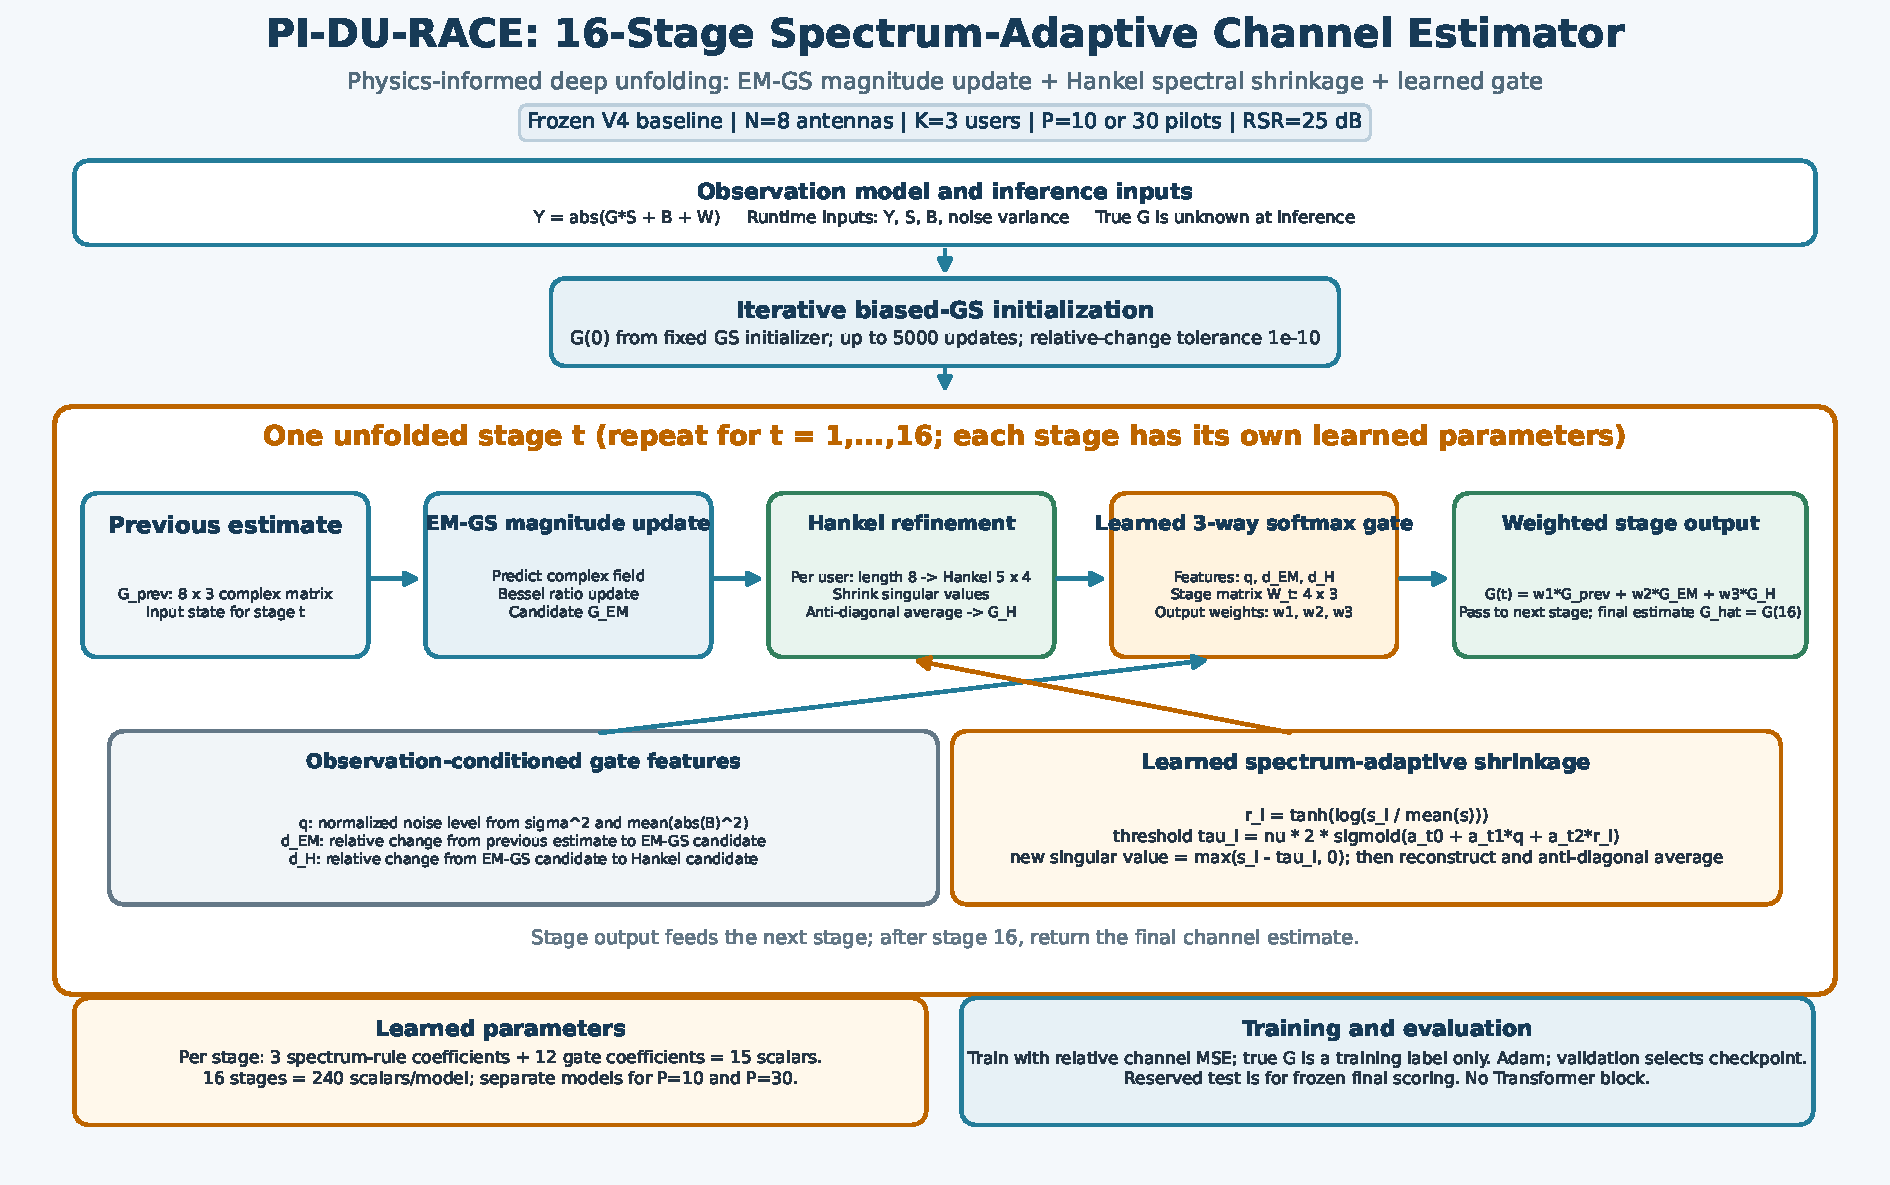
\includegraphics[width=\linewidth,height=0.88\textheight,keepaspectratio]{PI_DU_RACE_16Stage_Architecture.pdf}
\caption{Frozen V4 PI-DU-RACE architecture. Each of the 16 stages combines the previous estimate, the EM-GS candidate, and the spectrum-shrunk Hankel candidate using a learned three-way softmax gate.}
\label{fig:pidurace-architecture}
\end{figure}
\end{landscape}

\clearpage

\end{document}


